\begin{pastexam}[label={px:ccu-113-swa-07}]{中正資工所甲組 113 學年度 第 7 題}
（單選）

(3\%) Determine the binary tree using the provided in-order and post-order traversals. What is the resulting pre-order traversal of the constructed binary tree?

In-order：A, B, G, E, D, I, J, F, H, C

Post-order：\ G, E, J, I, H, F, D, C, B, A
\begin{enumerate}[label=\Alph*.]
\item A, B, C, D, E, F, G, I, H, J
\item A, B, G, E, D, C, I, J, F, H
\item A, B, C, D, E, G, F, I, J, H
\item A, B, C, D, E, F, G, I, J, H
\item None of the above
\end{enumerate}
\end{pastexam}

\begin{pastsoln}
答案是 C。

做法照資結書第~7.4~節：後序的最後一個是根，在中序裡找到根，左邊是左子樹、右邊是右子樹；後序裡左子樹的節點個數和中序
一樣，照個數切開，兩邊遞迴。 下面每一步寫「中序｜後序 $\Rightarrow$ 根」：
\begin{enumerate}
\item 全部：中序 A B G E D I J F H C｜後序 G E J I H F D C B \textbf{A}。 根 A；中序裡 A 在最前面，左子樹是空的，右子樹是
B G E D I J F H C（後序 G E J I H F D C B）。
\item B G E D I J F H C｜G E J I H F D C \textbf{B}。 根 B，左子樹空，右子樹是 G E D I J F H C（後序 G E J I H F D C）。
\item G E D I J F H C｜G E J I H F D \textbf{C}。 根 C，C 在中序最後，右子樹空，左子樹是 G E D I J F H（後序 G E J I H F D）。
\item G E D I J F H｜G E J I H F \textbf{D}。 根 D，左子樹 G E（後序 G E），右子樹 I J F H（後序 J I H F）。
\item 左邊 G E｜G \textbf{E}：根 E，G 在中序裡在 E 的左邊，是左子節點。
\item 右邊 I J F H｜J I H \textbf{F}：根 F，左子樹 I J（後序 J I），右子樹 H。
\item I J｜J \textbf{I}：根 I，J 在中序裡在 I 的右邊，是 I 的右子節點。
\end{enumerate}
\begin{center}
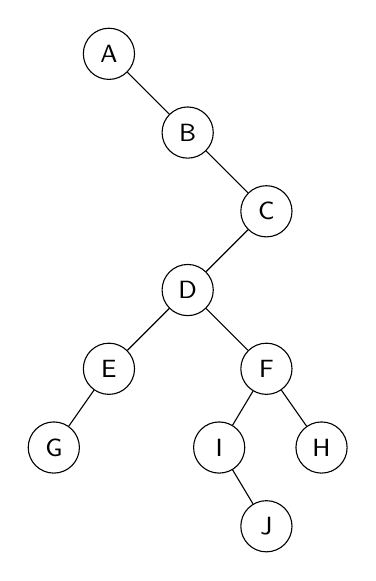
\begin{tikzpicture}[v/.style={circle,draw,minimum size=6.5mm,inner sep=0pt,font=\sffamily\small}]
\node[v] (A) at (0,0) {A};
\node[v] (B) at (1,-1) {B};
\node[v] (C) at (2,-2) {C};
\node[v] (D) at (1,-3) {D};
\node[v] (E) at (0,-4) {E};
\node[v] (F) at (2,-4) {F};
\node[v] (G) at (-0.7,-5) {G};
\node[v] (I) at (1.4,-5) {I};
\node[v] (H) at (2.7,-5) {H};
\node[v] (J) at (2,-6) {J};
\draw (A) -- (B); \draw (B) -- (C); \draw (C) -- (D);
\draw (D) -- (E); \draw (D) -- (F); \draw (E) -- (G);
\draw (F) -- (I); \draw (F) -- (H); \draw (I) -- (J);
\end{tikzpicture}
\end{center}
檢查：這棵樹的中序是 A B G E D I J F H C、後序是 G E J I H F D C B A，和題目一樣。 前序（根、左、右）：A，B，C，然後 C 的
左子樹 D、E、G、F、I、J、H，得到 $(A, B, C, D, E, G, F, I, J, H)$，就是 C。

逐項檢查：
\begin{itemize}
\item A：D 之後是 E、F，但 E 的子樹（G）要在走 D 的右子樹 F 之前走完；最後的 H、J 也反了，J 在 I 底下，前序要緊接在 I 後面。 錯。
\item B：A B 之後是 G，但 B 唯一的子節點是 C。 錯。
\item C：上面的結果。 對。
\item D：E 之後直接是 F，漏了 E 的左子節點 G 要先走。 錯。
\item E：C 是對的。 錯。
\end{itemize}
\end{pastsoln}
